\documentclass[12pt, a4paper]{article}
\title{Изучение плазмы газового разряда в неоне (3.5.1)}
\author{Стеценко Георгий, Б02-312}
\date{}
% !TeX encoding = UTF-8

\usepackage{geometry}
\usepackage{amsmath, amsfonts, amssymb, amsthm} % стандартный набор AMS-пакетов для математ. текстов
\usepackage{mathtext}
\usepackage[utf8]{inputenc} % кодировка utf8
\usepackage[russian]{babel} % русский язык
\usepackage[pdftex,dvipsnames]{xcolor} % работа с цветами
\usepackage[pdftex]{graphicx} % графика (картинки)
\usepackage{tikz,pgfplots} % рисунки
\usepackage{indentfirst}
%\usepackage[labelfont=bf,labelsep=endash,skip=3pt]{caption} % подпись картинок
% \usepackage{fancyhdr,pageslts} % настройка колонтитулов
\usepackage{enumitem} % работа со списками
\usepackage{floatrow,multicol,multirow,longtable,hhline} % работа с таблицами
\usepackage{float,wrapfig} % плавающие объекты
\usepackage{tcolorbox} % рамка вокруг текста
%\usepackage[calc]{datetime2} % дата
\usepackage{bm} % жирное начертание в формулах
\usepackage{physics} % физический пакет
\DeclareMathAlphabet\mathbfcal{OMS}{cmsy}{b}{n}
\usepackage{pgfornament} % красивые рюшечки и вензеля
\usepackage{mdframed}
\usepackage{derivative}
\usepackage{mathrsfs} %EDS
\usepackage{soul} % strikethorugh
%\usepackage{boondox-cal}

% ----------------------------------------
% Настройка шрифта

% Просто закооментируйте следующую строчку, если не работает. Будет другой шрифт, правда :(
% \usepackage{pscyr}

% ----------------------------------------
% Стилевые настройки

\usepackage{boldline} % жирная линия после таблиц (чтобы не было ошибок, этот пакет должен подключаться именно тут!)
\floatsetup[table]{style=Plaintop,floatrowsep=qquad} % настройка оформления таблиц
\setlist[enumerate,itemize]{leftmargin=5mm,itemindent=10mm,itemsep=0mm,
listparindent=0em,labelsep=2mm,topsep=2mm,labelwidth=4mm} % настройки списков

\setlength{\columnsep}{0.5cm} % расстояние между колонками
\setlength{\parskip}{1pt} % расстояние до текста от колонтитула

%\usepackage{titlesec} % управление оформлением section
%\renewcommand{\thesection}{\Roman{section}}
%\titleformat{\section}[block]{\bfseries\large}{\thesection.}{5pt}{}

% ----------------------------------------
% Настройки полей
\geometry{
  left=10mm,
  top=10mm,
  right=10mm,
  bottom=15mm,
  marginparsep=0mm,
  marginparwidth=0mm,
  headheight=0pt,
  headsep=0pt,
footskip=20pt}

% ----------------------------------------
% Настройки колонтитулов и нумерации страниц
\pagenumbering{arabic}



\newcounter{ntask}
\setcounter{ntask}{0}


\newcommand{\arsh}{\mathrm{arsh} \,\,}
\newcommand{\arch}{\mathrm{arch} \,\,}
\newcommand{\arth}{\mathrm{arth} \,\,}
\newcommand{\arcth}{\mathrm{arcth} \,\,}
\renewcommand{\Re}{\operatorname{Re} \,}
\newcommand{\EDS}{\mathscr{E}}
\newcommand{\diffract}[1]{\frac{\mathrm{d}#1}{\mathrm{d}t}}

\newcommand{\kHz}{~\mathrm{kHz}}
\newcommand{\us}{~\mathrm{\mu s}}
\addto\captionsrussian{\def\refname{Источники}}

\begin{document}
	\maketitle
	
	\section{Цель работы} 
Изучение вольт-амперной характеристики тлеющего разряда, изучение свойств плазмы методом зондовых характеристик.



\section{Теоретические сведения}
\subsection{Плазма}
В ионизированном газе поле ионов <<экранируется>> электронами. Для поля $\mathbf{E}$ и плотности $\rho$ электрического заряда
$$
\text{div}~\mathbf{E} = 4 \rho / \varepsilon_0,
$$
а с учётом сферической симметрии и $\mathbf{E} = -\text{grad}~\varphi$:
\begin{equation}
\dfrac{d^2 \varphi}{dr^2}+\dfrac{2}{r}\dfrac{d\varphi}{dr}=-4\pi \rho.
\end{equation}
Плотности заряда электронов и ионов (которые мы считаем бесконечно тяжёлыми и поэтому неподвижными)
\begin{equation}
\begin{array}{c}
\rho_e = -ne \cdot \exp\left(\dfrac{e\varphi}{kT_e}\right),\\
\rho_i = ne.
\end{array}
\end{equation}
Тогда из $(1)$ в предположении $\dfrac{e\varphi}{kT_e} \ll 1$ получим
\begin{equation}
\varphi = \dfrac{Ze}{r}e^{-r/r_D},
\end{equation}
где $r_D = \sqrt{\dfrac{\varepsilon_0 kT_e}{n e^2}}$ -- \textit{радиус Дебая}. Среднее число ионов в сфере такого радиуса  

\begin{equation}
N_D = n\dfrac{4}{3}\pi r_D^2.
\end{equation}
Теперь выделим параллелепипед с плотностью $n$ электронов, сместим их на $x$. Возникнут поверхностные заряды $\sigma = nex$, поле от которых будет придавать электронам ускорение:
$$
\dfrac{d^2x}{dt^2}=-\dfrac{eE}{m}=-\dfrac{n e^2}{m \varepsilon_0}x.
$$ 
Отсюда получаем \textit{плазменную (ленгмюровскую) частоту} колебаний электронов:
\begin{equation}
\omega_p = \sqrt{\dfrac{4\pi ne^2}{m \varepsilon_0}}.
\end{equation}
\subsection{Одиночный зонд}
При внесении в плазму уединённого проводника -- \textit{зонда} -- с потенциалом, изначально равным потенциалу точки плазмы, в которую его помещают, на него поступают токи электроннов и ионов:
\begin{equation}
\begin{array}{c}
I_{e0} = \dfrac{n \langle v_e \rangle}{4}eS,\\
I_{i0} = \dfrac{n \langle v_i \rangle}{4}eS,
\end{array}
\end{equation}
где $\langle v_e \rangle$ и $\langle v_i \rangle$ -- средние скорости электронов и ионов, $S$ -- площадь зонда, $n$ -- плотность электронов и ионов. Скорости электронов много больше скорости ионов, поэтому $I_{i0} \ll I_{e0}$. Зонд будет заряжаться до некоторого равновестного напряжения $-U_f$ -- \textit{плавающего потенциала}.

\begin{wrapfigure}[8]{r}{5.5cm}\vspace{0}
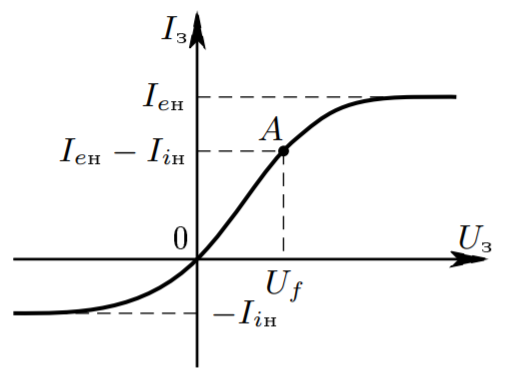
\includegraphics[scale=0.5]{pics/3.png}
\end{wrapfigure}  
В равновесии ионный ток мало меняется, а электронный имеет вид
$$
I_e = I_0 \exp\left( -\dfrac{eU_f}{kT_e} \right).
$$
Будем подавать потенциал $U_\text{з}$ на зонд и снимать значение зондового тока $I_\text{з}$. Максимальное значение тока $I_{e\text{н}}$ -- электронный ток насыщения, а минимальное $I_{i\text{н}}$ -- ионный ток насыщения. Значение из эмпирической формулы Бомона:
\begin{equation}
I_{i\text{н}} = 0.4 neS \sqrt{\dfrac{2kT_e}{m_i}}.
\label{bomond}
\end{equation}
\subsection*{Двойной зонд}
Двойной зонд -- система из двух одинаковых зондов, расположенных на небольшом расстоянии друг от друга, между которыми создаётся разность потенциалов, меньшая $U_f$. Рассчитаем ток между ними вблизи $I=0$. При небольших разностях потенциалов ионные токи на оба зонда близки к току насыщения и компенсируют друг друга, а значит величина результирующего тока полностью связана с разностью электронных токов. Пусть потенциалы на зондах
$$
U_1 = -U_f + \Delta U_1,
$$
$$
U_2 = -U_f + \Delta U_2.
$$
Между зондами $U = U_2 - U_1 = \Delta U_2 - \Delta U_1$.
Через первый электрод
\begin{equation}
I_1 = I_{i\text{н}} + I_{e1} = I_{i\text{н}} - \dfrac{1}{4}neS\langle v_e\rangle \exp\left(-\dfrac{eU_f}{kT_e}\right)\exp\left(\dfrac{e\Delta U_1}{kT_e}\right)=I_{i\text{н}}\left(1 - \exp\left( \dfrac{e\Delta U_1}{kT_e} \right)\right).
\end{equation}
Аналогично через второй получим
\begin{equation}
I_2 = I_{i\text{н}}\left(1 - \exp\left( \dfrac{e\Delta U_2}{kT_e} \right)\right)
\end{equation}
  
Из $(7)$ и $(8)$ с учётом последовательного соединение зондов ($I_1 = -I_2 = I)$:
$$
\Delta U_1= \dfrac{kT_e}{e}\text{ln}\left(1 - \dfrac{I}{I_{i\text{н}}}\right)
$$
$$
\Delta U_2= \dfrac{kT_e}{e}\text{ln}\left(1 + \dfrac{I}{I_{i\text{н}}}\right)
$$

Тогда итоговые формулы для разности потенциалов и тока

\begin{equation}
U = \dfrac{kT_e}{e}\text{ln}\dfrac{1 - I/I_{i\text{н}}}{1 + I/I_{i\text{н}}}, 
I = I_{i\text{н}} \text{th}\dfrac{eU}{2kT_e}.
\end{equation}
Реальная зависимость выглядит несколько иначе и описывается формулой 


\begin{equation}
I = I_{i\text{н}} \text{th}\dfrac{eU}{2kT_e} + AU.
\end{equation}


\section{Методика измерений и результаты}
\textbf{В работе используются:} стеклянная газоразрядная трубка, наполненная изотопом неона, высоковольтный источник питания (ВИП), источник питания постоянного тока, делитель напряжения, резистор, потенциометр, амперметры, вольтметры, переключатели.

\section*{Описание установки}
\begin{center}
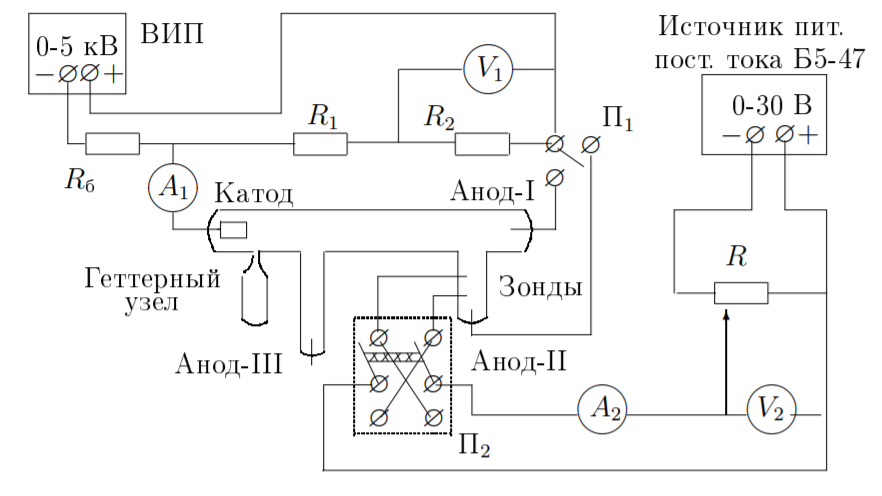
\includegraphics[scale=0.6]{pics/1.png}
\end{center}
Стеклянная газоразрядная трубка имеет холодный (ненакаливаемый) полый катод, три анода и \textit{геттерный} узел -- стеклянный баллон, на внутреннюю повехность которого напылена газопоглощающая плёнка (\textit{геттер}). Трубка наполнена изотопом неона $^22$Ne при давлении 2 мм рт. ст. Катод и один из анодом (I и II) с помощью переключателя $\Pi_1$ подключается через балластный резистор $R_\text{б}$ ($\approx 450~\mathrm{k\Omega}$) к регулируемому ВИП с выкодным напряжением до 5 кВ.\\
При подключении к ВИП анода-I между ним и катодом возникает газовый разряд. Ток разряда измеряется миллиамперметром $A_1$, а падение напряжения на разрядной трубке -- цифровым вольтметром $V_1$, подключённым к трубке через высокоомный ($25~\mathrm{M\Omega}$) делитель напряжения с коэффициентом $(R_1+R_2)/R_2 = 10$.\\
С учётом конечного сопротивления вольтметра $R_V = 10~\mathrm{M\Omega}$, он показывает заниженные по сравнению с ожидамыми в $\alpha = 12.3$ раз.
При подключении к ВИП анода-II разряд возникает в пространстве между катодом и анодом-II, где находятся двойной зонд, используемый для диагностики плазмы положительного столба. Зонды изготовлены из молибденовой проволоки диаметром $d = 0.2$ мм и имеют длину $l = 5.2$ мм. Они подключены к источнику питания GPS через потенциометр $R$. Переключатель $\Pi_2$ позволяет изменять полярность напряжения на зондах. Величина напряжения на зондах изменяеься с помощью дискретного переключателя <<$V$>> выходного напряжения источника питания и потенциометра $R$, а измеряется цифровым вольтметром $V_2$. Для измерения зондового тока используется мультиметр $A_2$.

В работе имеются следующие части: определение напряжения зажигания и гашения, снятие ВАХ, снятие зондовых характеристик.

\section{Результаты измерений}

Найдём для начала напряжение зажигания:

\begin{table}[H]
\begin{tabular}{|l|lllll|}
\hline
$V_\text{ign}$     & \multicolumn{1}{l|}{203} & \multicolumn{1}{l|}{201} & \multicolumn{1}{l|}{199} & \multicolumn{1}{l|}{196} & 202 \\ \hline
$V_\text{ign.avg}$ & \multicolumn{5}{c|}{200}                                                                                        \\ \hline
\end{tabular}
\end{table}

Теперь снимем ВАХ катод-анод на увеличение и падение тока и построим её график.
\begin{table}[H]
\tiny
\begin{tabular}{|r|c|c|c|c|c|c|c|c|c|c|c|c|c|c|c|c|}
\hline
$I$, mA                         & 0,508 & 0,808 & 1,107 & 1,400 & 1,723 & 2,007 & 2,357 & 2,604 & 2,928 & 3,207 & 3,500 & 3,934 & 4,110 & 4,451 & 4,723 & 5,019 \\ \hline
\multicolumn{1}{|l|}{$U_V$, V} & 35,15 & 34,17 & 32,51 & 28,56 & 26,19 & 24,86 & 23,56 & 22,73 & 21,63 & 20,84 & 20,39 & 20,03 & 19,81 & 19,4  & 19,22 & 18,96 \\ \hline
$U$, V                          & 430,6 & 418,6 & 398,2 & 349,9 & 320,8 & 304,5 & 288,6 & 278,4 & 265,0 & 255,3 & 249,8 & 245,4 & 242,7 & 237,7 & 235,4 & 232,3 \\ \hline
$I$, mA                         & 5,019 & 4,705 & 4,349 & 4,11  & 3,782 & 3,504 & 3,202 & 2,893 & 2,59  & 2,305 & 1,999 & 1,689 & 1,33  & 1,03  & 0,807 & 0,374 \\ \hline
\multicolumn{1}{|l|}{$U_V$, V} & 18,96 & 19,2  & 19,48 & 19,82 & 20,14 & 20,22 & 20,75 & 21,68 & 22,75 & 23,62 & 24,78 & 26,3  & 29,35 & 32,63 & 34,15 & 35,6  \\ \hline
$U$, V                          & 232,3 & 235,2 & 238,6 & 242,8 & 246,7 & 247,7 & 254,2 & 265,6 & 278,7 & 289,3 & 303,6 & 322,2 & 359,5 & 399,7 & 418,3 & 436,1 \\ \hline
\end{tabular}
\end{table}

\begin{figure}[H]
    \centering
    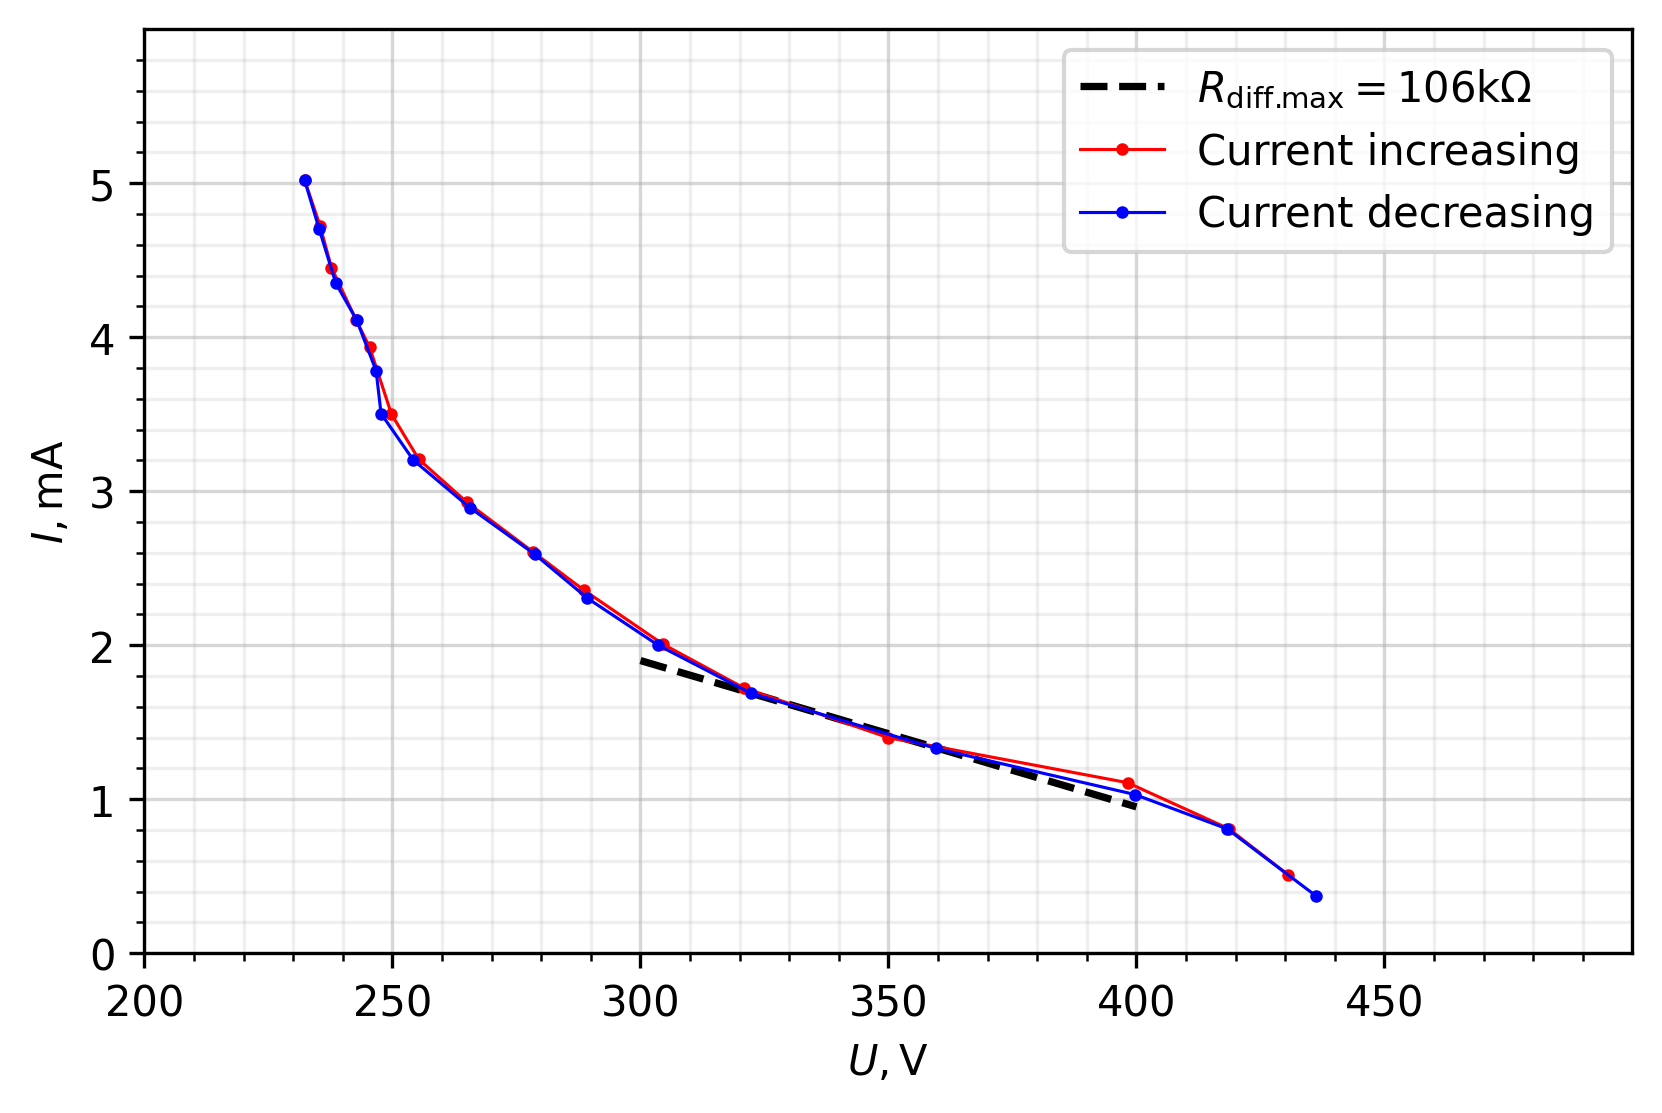
\includegraphics[width = 0.8\linewidth]{pics/CVD.png}
    \caption{ВАХ катод-анод} 
\end{figure}
По минимальному углу наклона так же найдём максимальное дифференциальное сопротивление $R_\text{dif} = 106 \mathrm{k\Omega}$.

Теперь снимем зондовые характеристики для анодных токов $5~\mathrm{mA}$, $3.0~\mathrm{mA}$, $1. 5~\mathrm{mA}$ (см. приложение). По полученным данным построим график \ref{amplot}. На график, кроме того, нанесены аппроксимации функциями вида $A\cdot\tanh (BU) + C\cdot U + D$. Выпишем получившиеся параметры аппроксимации:
% Please add the following required packages to your document preamble:
% \usepackage{multirow}
\begin{table}[H]
\begin{tabular}{|r|l|l|l|l|}
\hline
                        & A, \mathrm{uA} & B, \mathrm{1/V} & C, \mathrm{uA/V} & D, \mathrm{uA} \\ \hline
\multirow{2}{*}{5 mA}   & 84.8           & 0.133           & 1.37             & -6.45          \\ \cline{2-5} 
                        & $\pm$8.5       & $\pm$0.014      & $\pm$0.39        & $\pm$0.79      \\ \hline
\multirow{2}{*}{3 mA}   & 55.6           & 0.122           & 0.51             & -4.07          \\ \cline{2-5} 
                        & $\pm$2.5       & $\pm$0.005      & $\pm$0.11        & $\pm$0.19      \\ \hline
\multirow{2}{*}{1.5 mA} & 27.0           & 0.132           & 0.316            & -2.37          \\ \cline{2-5} 
                        & $\pm$0.6       & $\pm$0.003      & $\pm$0.028       & $\pm$0.55      \\ \hline
\end{tabular}
\end{table}

\begin{figure}[]
\centering
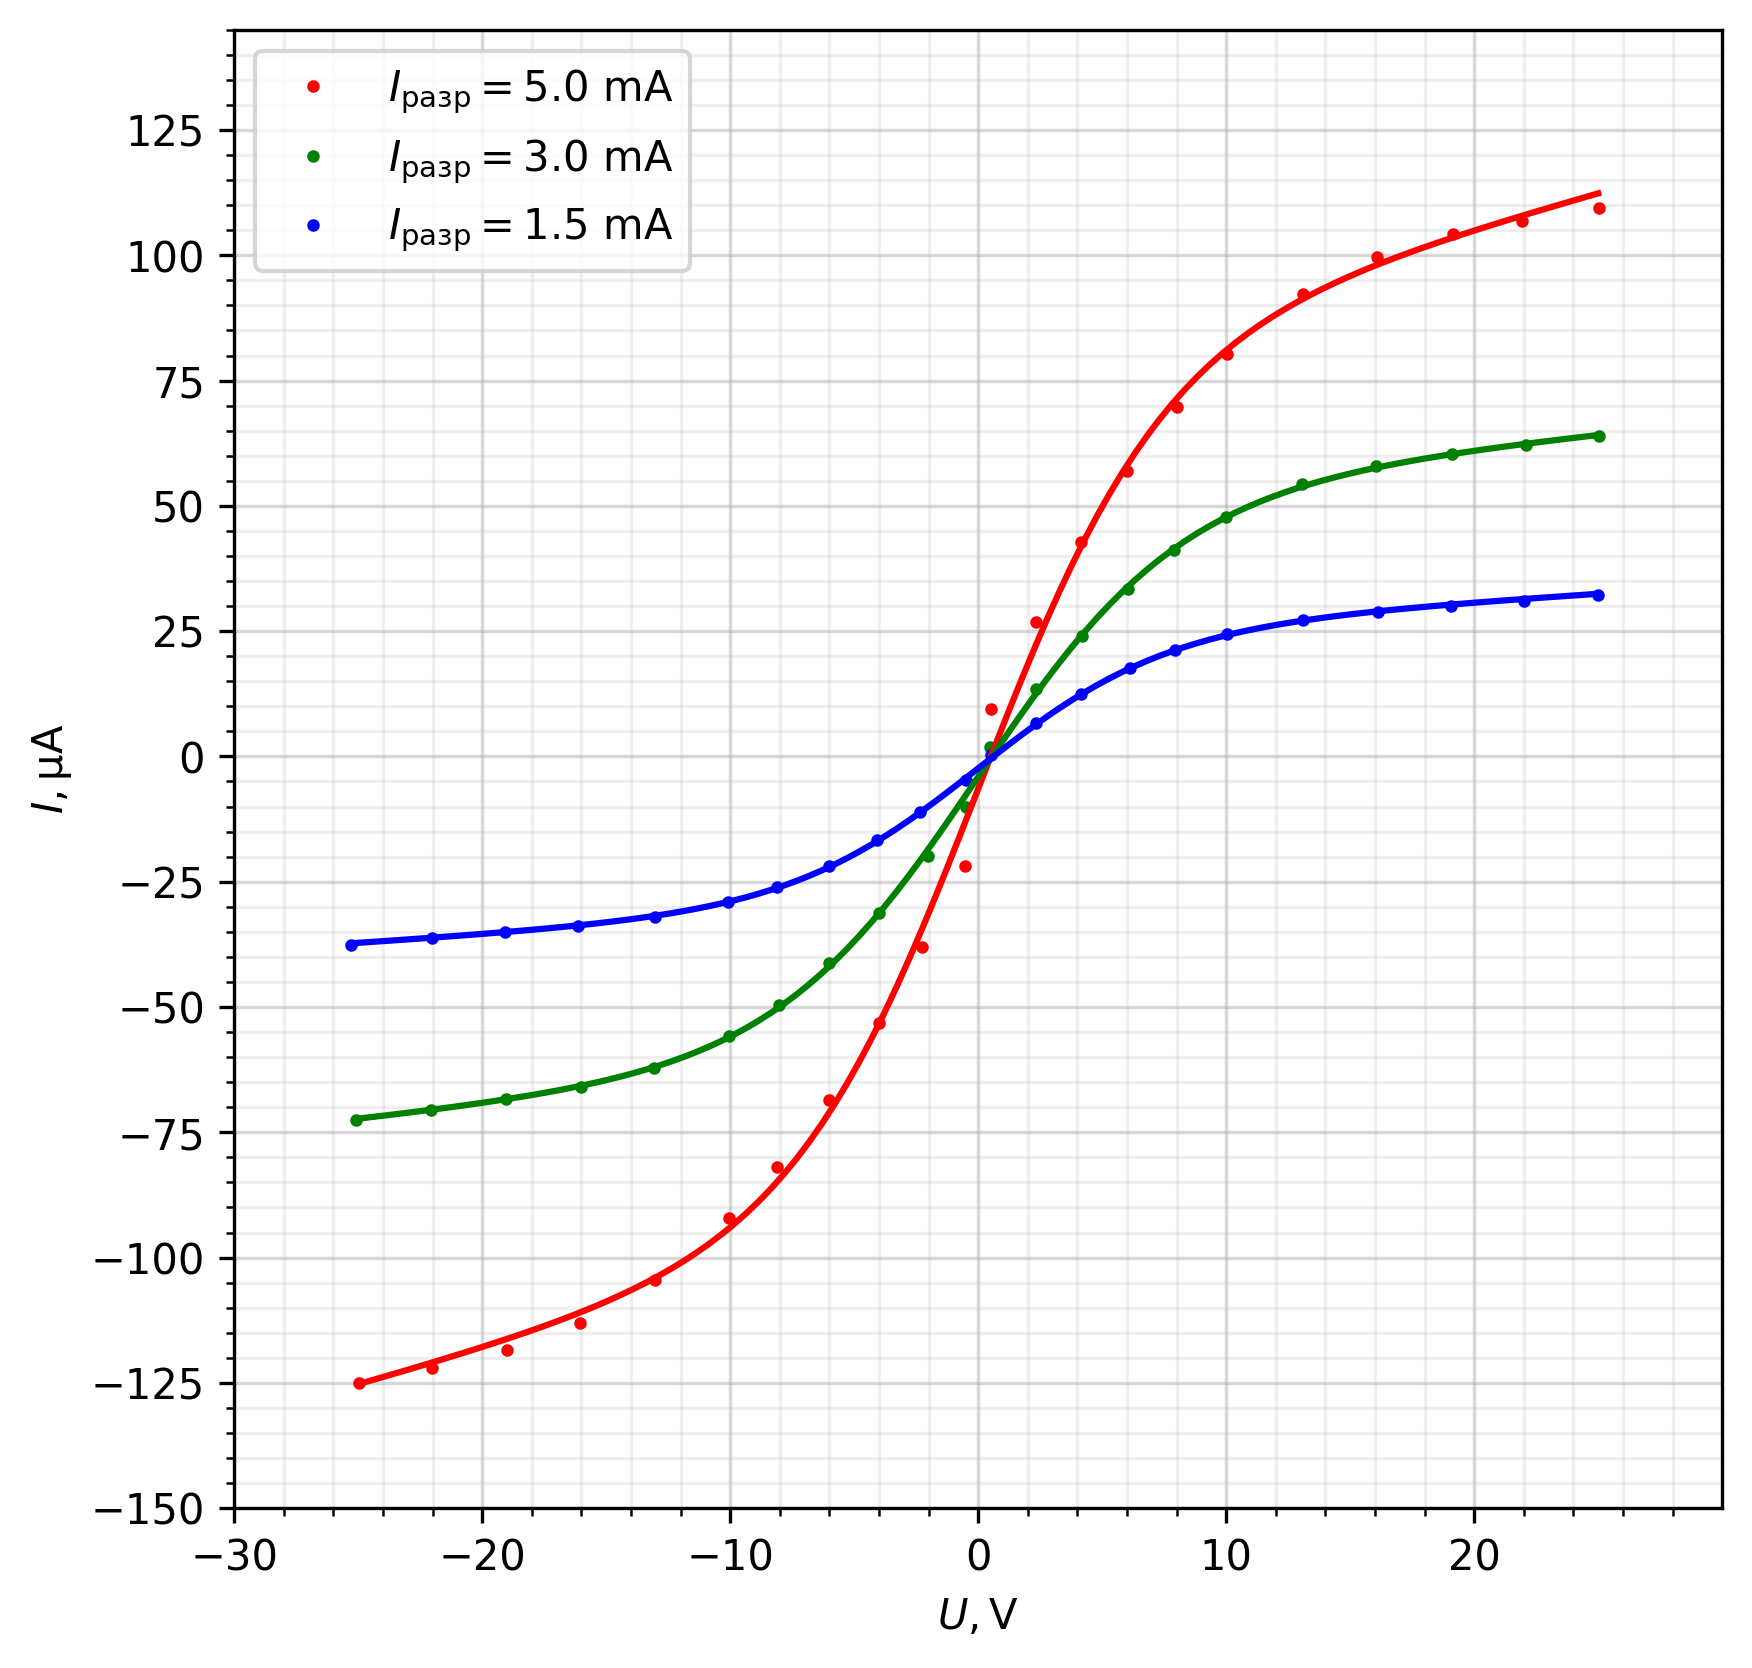
\includegraphics[width=0.6\linewidth]{pics/zond}
\caption{Зондовая характеристика}
\label{amplot}
\end{figure}

Поймём, что по сути своей $A = I_\text{и.н.}$, $B = \frac{e}{2kT_e}$.
$$kT_{e1} = \frac{1}{2\cdot0.133} \mathrm{eV}\approx(3.8\pm0.4) \mathrm{eV}$$
$$kT_{e2} = \frac{1}{2\cdot0.122} \mathrm{eV}\approx(4.1\pm0.2) \mathrm{eV}$$
$$kT_{e3} = \frac{1}{2\cdot0.132} \mathrm{eV}\approx(3.8\pm0.1) \mathrm{eV}$$
\newpage
Пользуясь (\ref{bomond}), найдём концентрацию ионов в плазме.
$$n_{1i} = 6.7\cdot 10^{16}~\mathrm{m}^{-3}$$
$$n_{2i} = 6.5\cdot 10^{16}~\mathrm{m}^{-3}$$
$$n_{3i} = 6.7\cdot 10^{16}~\mathrm{m}^{-3}$$.

В общем и целом ионная концентрация остается почти одинаковой. Это согласуется со свойством самоорганизации нормального тлеющего разряда -- ток в нем растёт за счёт увеличения размеров катодного пятна, при этом концентрация носителей остается неизменной. Примем $n_{ср} = 6.6\cdot 10^{16}~\mathrm{m}^{-3}$. Тогда так как концентрация неионизованных частиц $n = 6.4 \cdot 10^{22}~\mathrm{m}^{-3}$, степень ионизации $\alpha \sim 10^{-6}$.

Найдём теперь дебаевский радиус
$$r_D = 58.4 \mathrm{\mu m}$$
и количество ионов в дебаевской ячейке
$$N_i = {n_i} \cdot {4/3 \pi r_D ^3} = 56000 \geq 1$$
что означает, что плазму можно считать идеальной.

\section{Обусждение результатов и выводы}
В ходе работы были сняты вольтамперные и зондовые характеристики тлеющего разряда, обнаружена большая разница в температурах ионов и электронов в нем ($T_e \sim 40000 \mathrm{K}$), независимость концентрации носителей заряда от величины анодного тока, вычислен дебаевский радиус и показано, что плазму можно считать идеальной. Полученные результаты хорошо качественно согласуются с теорией. 
\newpage
\section{Приложение}
\begin{table}[H]
\begin{tabular}{|rr|rr|rr|}
\hline
\multicolumn{2}{|l|}{5 mA}                                  & \multicolumn{2}{l|}{3 mA}                                  & \multicolumn{2}{l|}{1.5 mA}                                \\ \hline
\multicolumn{1}{|l|}{U_з, V} & \multicolumn{1}{l|}{I_з, uA} & \multicolumn{1}{l|}{U_з, V} & \multicolumn{1}{l|}{I_з, uA} & \multicolumn{1}{l|}{U_з, V} & \multicolumn{1}{l|}{I_з, uA} \\ \hline
\multicolumn{1}{|r|}{25,05}  & 109,50                       & \multicolumn{1}{r|}{25,05}  & 63,94                        & \multicolumn{1}{r|}{25,01}  & 32,22                        \\ \hline
\multicolumn{1}{|r|}{21,94}  & 106,90                       & \multicolumn{1}{r|}{22,08}  & 62,12                        & \multicolumn{1}{r|}{22,02}  & 31,10                        \\ \hline
\multicolumn{1}{|r|}{19,16}  & 104,34                       & \multicolumn{1}{r|}{19,11}  & 60,28                        & \multicolumn{1}{r|}{19,07}  & 30,04                        \\ \hline
\multicolumn{1}{|r|}{16,07}  & 99,70                        & \multicolumn{1}{r|}{16,05}  & 57,94                        & \multicolumn{1}{r|}{16,14}  & 28,91                        \\ \hline
\multicolumn{1}{|r|}{13,08}  & 92,26                        & \multicolumn{1}{r|}{13,05}  & 54,32                        & \multicolumn{1}{r|}{13,09}  & 27,25                        \\ \hline
\multicolumn{1}{|r|}{10,03}  & 80,30                        & \multicolumn{1}{r|}{9,99}   & 47,80                        & \multicolumn{1}{r|}{10,05}  & 24,38                        \\ \hline
\multicolumn{1}{|r|}{8,00}   & 69,63                        & \multicolumn{1}{r|}{7,91}   & 41,15                        & \multicolumn{1}{r|}{7,92}   & 21,22                        \\ \hline
\multicolumn{1}{|r|}{6,01}   & 56,87                        & \multicolumn{1}{r|}{6,02}   & 33,39                        & \multicolumn{1}{r|}{6,11}   & 17,55                        \\ \hline
\multicolumn{1}{|r|}{4,16}   & 42,78                        & \multicolumn{1}{r|}{4,17}   & 24,03                        & \multicolumn{1}{r|}{4,16}   & 12,49                        \\ \hline
\multicolumn{1}{|r|}{2,33}   & 26,83                        & \multicolumn{1}{r|}{2,33}   & 13,43                        & \multicolumn{1}{r|}{2,33}   & 6,74                         \\ \hline
\multicolumn{1}{|r|}{0,51}   & 9,38                         & \multicolumn{1}{r|}{0,49}   & 1,81                         & \multicolumn{1}{r|}{0,51}   & 0,20                         \\ \hline
\multicolumn{1}{|r|}{-0,53}  & -21,83                       & \multicolumn{1}{r|}{-0,50}  & -10,08                       & \multicolumn{1}{r|}{-0,50}  & -4,61                        \\ \hline
\multicolumn{1}{|r|}{-2,25}  & -38,00                       & \multicolumn{1}{r|}{-2,04}  & -19,89                       & \multicolumn{1}{r|}{-2,33}  & -11,14                       \\ \hline
\multicolumn{1}{|r|}{-4,02}  & -53,26                       & \multicolumn{1}{r|}{-4,01}  & -31,31                       & \multicolumn{1}{r|}{-4,10}  & -16,76                       \\ \hline
\multicolumn{1}{|r|}{-6,02}  & -68,51                       & \multicolumn{1}{r|}{-6,02}  & -41,31                       & \multicolumn{1}{r|}{-6,02}  & -21,80                       \\ \hline
\multicolumn{1}{|r|}{-8,11}  & -81,92                       & \multicolumn{1}{r|}{-8,05}  & -49,52                       & \multicolumn{1}{r|}{-8,13}  & -26,07                       \\ \hline
\multicolumn{1}{|r|}{-10,03} & -92,10                       & \multicolumn{1}{r|}{-10,05} & -55,77                       & \multicolumn{1}{r|}{-10,09} & -29,01                       \\ \hline
\multicolumn{1}{|r|}{-13,02} & -104,39                      & \multicolumn{1}{r|}{-13,06} & -62,19                       & \multicolumn{1}{r|}{-13,04} & -31,96                       \\ \hline
\multicolumn{1}{|r|}{-16,05} & -113,00                      & \multicolumn{1}{r|}{-16,00} & -65,92                       & \multicolumn{1}{r|}{-16,14} & -33,80                       \\ \hline
\multicolumn{1}{|r|}{-19,00} & -118,50                      & \multicolumn{1}{r|}{-19,06} & -68,45                       & \multicolumn{1}{r|}{-19,08} & -35,10                       \\ \hline
\multicolumn{1}{|r|}{-22,03} & -122,12                      & \multicolumn{1}{r|}{-22,07} & -70,48                       & \multicolumn{1}{r|}{-22,01} & -36,30                       \\ \hline
\multicolumn{1}{|r|}{-24,98} & -125,00                      & \multicolumn{1}{r|}{-25,08} & -72,48                       & \multicolumn{1}{r|}{-25,30} & -37,70                       \\ \hline
\end{tabular}
\end{table}

\end{document}